\section{L'\algo}
\subsection{Le principe}
L'algorithme prend en entrée un graphe pondéré par des réels positifs et un sommet source. Il s'agit de construire progressivement un sous-graphe dans lequel sont classés les différents sommets par ordre croissant de leur distance minimale au sommet de départ. La distance correspond à la somme des poids des arcs empruntés.

Au départ, on considère que les distances de chaque sommet au sommet de départ sont infinies, sauf pour le sommet de départ pour lequel la distance est nulle. Le sous-graphe de départ est l'ensemble vide.

Au cours de chaque itération, on choisit en dehors du sous-graphe un sommet de distance minimale et on l'ajoute au sous-graphe. Ensuite, on met à jour les distances des sommets voisins de celui ajouté. La mise à jour s'opère comme suit : la nouvelle distance du sommet voisin est le minimum entre la distance existante et celle obtenue en ajoutant le poids de l'arc entre sommet voisin et sommet ajouté à la distance du sommet ajouté.
On continue ainsi jusqu'à épuisement des sommets (ou jusqu'à sélection du sommet d'arrivée).
\subsection{Schéma de l'algorithme}
Le graphe est noté  $G=(S,A)$ où :
\begin{itemize}
\item l'ensemble $S$ est l'ensemble fini des sommets du graphe $G$ ;
\item l'ensemble $A$ est l'ensemble des arcs de $G$ tel que : si $(s_{1},s_{2})$ est dans $A$, alors il existe un arc depuis le nœud $s_{1}$ vers le nœud $s_{2}$ ;

\item on définit la fonction \emph{poids} définie sur $S \times S$ dans $ \R^{+}\cup \{+\infty \}$ qui à un couple $(s_{1},s_{2})$ associe le poids positif \emph{$poids(s_{1},s_{2})$}  de l'arc reliant $s_{1}$ à $s_{2}$ (et $+\infty$ s'il n'y a pas d'arc reliant $s_{1}$ à $s_{2}$).
\end{itemize}
Le poids du chemin entre deux sommets est la somme des poids des arcs qui le composent. Pour une paire donnée de sommets $s_{deb}$ (le sommet du départ) $s_{fin}$ (le sommet d'arrivée) appartenant à $S$, l'algorithme trouve un chemin depuis $s_{deb}$ vers $s_{fin}$ de moindre poids (autrement dit un chemin le plus léger ou encore le plus court).

L'algorithme fonctionne en construisant un sous-graphe $P$ de manière que la distance entre un sommet $s$  de $P$ depuis $s_{deb}$ soit connue et soit un minimum dans $G$. Initialement, $P$ contient simplement le nœud $s_{deb}$ isolé, et la distance de $s_{deb}$ à lui-même vaut zéro. Des arcs sont ajoutés à $P$ à chaque étape :
\begin{enumerate}
\item en identifiant tous les arcs $a_{i}=(s_{i1},s_{i2})$ dans $P\times G$;
\item en choisissant l'arc $a_{j}=(s_{j1},s_{j2})$ dans $P\times G$ qui donne la distance minimum depuis $S_{deb}$  à $s_{j2}$ en passant tous les chemins créés menant à ce nœud.
\end{enumerate}
L'algorithme se termine soit quand $P$ devient un arbre couvrant de $G$, soit quand tous les nœuds d'intérêt sont dans $P$.
Information tiré de~\cite{dijkstra.algo.wiki}.
\subsection{L'\algo en C++}
On voit à la figure~\ref{algo_code} une implementation du code en C++
\begin{figure}[!htb]
\lstinputlisting[
    language=C++,
    style=myStyle,
]{dijkstra.cpp}
\caption{L'\algo en C++}\label{algo_code}
\end{figure}

\subsection{Exemple graphique}
\begin{figure}[!htb]
\centering
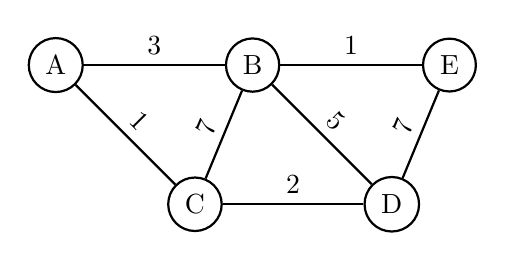
\begin{tikzpicture}[node distance={25mm}, thick, main/.style = {draw, circle}]
\node[main] (1) {A};
\node[main] (2) [right of=1] {B};
\node[main] (3) [below right of=1] {C};
\node[main] (4) [below right of=2] {D};
\node[main] (5) [right of=2] {E};

\draw (1) -- node[midway, above, pos=0.5] {3} (2);
\draw (1) -- node[midway, above, sloped, pos=0.5] {1} (3);
\draw (2) -- node[midway, above, sloped, pos=0.5] {7} (3);
\draw (3) -- node[midway, above , pos=0.5] {2} (4);
\draw (2) -- node[midway, above, sloped, pos=0.5] {5} (4);
\draw (2) -- node[midway, above , pos=0.5] {1} (5);
\draw (4) -- node[midway, above, sloped, pos=0.5] {7} (5);
\end{tikzpicture}
\caption{Graphe d'exemple}
\label{graphbase}
\end{figure}
Supposons le graphe pondéré de la figure~\ref{graphbase}.

Pendant l'exécution de l'algorithme, nous allons marquer chaque nœud avec sa
distance minimale au nœud C (notre nœud sélectionné). Pour le noeud C, cette
distance est 0. Pour le reste des noeuds, comme nous ne connaissons pas encore
cette distance minimale, elle commence à l'infinie ($\infty$).
Nous aurons également un noeud courant. Initialement, nous le définissons sur C
(notre nœud sélectionné). Dans l'image, nous marquons le nœud actuel avec un
point rouge. Regardez la figure~\ref{fig:all_inf}.

\begin{figure}[!htb]
\centering
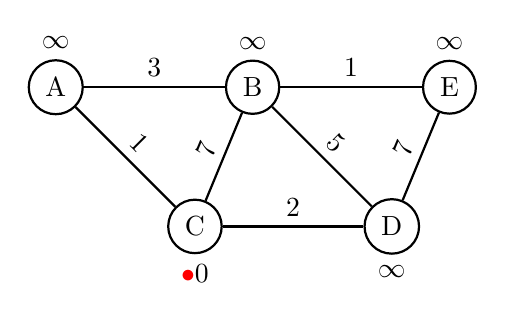
\begin{tikzpicture}[node distance={25mm}, thick, main/.style = {draw, circle}]
\node[main, label=above:{$\infty$}] (1) {A};
\node[main, label=above:{$\infty$}] (2) [right of=1] {B};
\node[main, label=below:{$\textcolor{red}{\bullet} 0$}] (3) [below right of=1] {C};
\node[main, label=below:{$\infty$}] (4) [below right of=2] {D};
\node[main, label=above:{$\infty$}] (5) [right of=2] {E};
\draw (1) -- node[midway, above, pos=0.5] {3} (2);
\draw (1) -- node[midway, above, sloped, pos=0.5] {1} (3);
\draw (2) -- node[midway, above, sloped, pos=0.5] {7} (3);
\draw (3) -- node[midway, above , pos=0.5] {2} (4);
\draw (2) -- node[midway, above, sloped, pos=0.5] {5} (4);
\draw (2) -- node[midway, above , pos=0.5] {1} (5);
\draw (4) -- node[midway, above, sloped, pos=0.5] {7} (5);
\end{tikzpicture}
\caption{Etape 1}\label{fig:all_inf}
\end{figure}

Maintenant, vérifions les voisins de notre nœud actuel (A, B et D) sans ordre particulier. Commençons par B. Nous ajoutons la distance minimale du nœud actuel (dans ce cas, 0) au poids de l'arête qui relie notre nœud actuel à B (dans ce cas, 7), et nous obtenons 0 + 7 = 7. Nous comparons cette valeur avec la distance minimale de B (infini); la valeur la plus petie est celle qui reste comme distance minimale de B (dans ce cas, 7 est plus pétit que l'infini) et ainsi de suite pour les autres voisins.

Nous avons vérifié tous les voisins de C. Pour cette raison, on le marque comme visité.

Nous devons maintenant choisir un nouveau noeud courant. Ce noeud doit être le noeud non visité avec la plus petite distance minimale (donc, le noeud avec le plus petit nombre et sans marque de contrôle). C'est A. Marquons-le d'un point rouge. Regardez la figure~\ref{fig:etp_2}.
\begin{figure}[!htb]
\centering
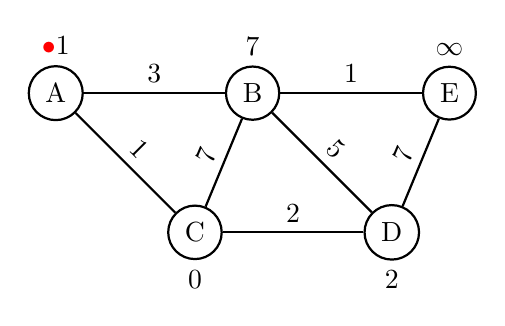
\begin{tikzpicture}[node distance={25mm}, thick, main/.style = {draw, circle}]
\node[main, label=above:{$\textcolor{red}{\bullet}1$}] (1) {A};
\node[main, label=above:{$7$}] (2) [right of=1] {B};
\node[main, label=below:{$\textcolor{green}{\checkmark} 0$}] (3) [below right of=1] {C};
\node[main, label=below:{$2$}] (4) [below right of=2] {D};
\node[main, label=above:{$\infty$}] (5) [right of=2] {E};
\draw (1) -- node[midway, above, pos=0.5] {3} (2);
\draw (1) -- node[midway, above, sloped, pos=0.5] {1} (3);
\draw (2) -- node[midway, above, sloped, pos=0.5] {7} (3);
\draw (3) -- node[midway, above , pos=0.5] {2} (4);
\draw (2) -- node[midway, above, sloped, pos=0.5] {5} (4);
\draw (2) -- node[midway, above , pos=0.5] {1} (5);
\draw (4) -- node[midway, above, sloped, pos=0.5] {7} (5);
\end{tikzpicture}
\caption{Etape 2}\label{fig:etp_2}
\end{figure}

Et maintenant nous répétons l'algorithme. Nous vérifions les voisins de notre nœud actuel, en ignorant les nœuds visités. Cela signifie que nous ne vérifions que B.

Pour B, nous ajoutons 1 (la distance minimale de A, notre noeud actuel) à 3 (le poids de l'arête reliant A et B) pour obtenir 4. Nous comparons ce 4 avec la distance minimale de B (7) et nous laissons la plus petite valeur : 4. Regardez la figure~\ref{fig:etp_3}.

\begin{figure}[!htb]
\centering
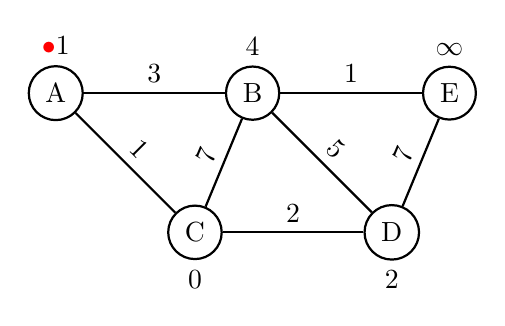
\begin{tikzpicture}[node distance={25mm}, thick, main/.style = {draw, circle}]
\node[main, label=above:{$\textcolor{red}{\bullet}1$}] (1) {A};
\node[main, label=above:{$4$}] (2) [right of=1] {B};
\node[main, label=below:{$\textcolor{green}{\checkmark} 0$}] (3) [below right of=1] {C};
\node[main, label=below:{$2$}] (4) [below right of=2] {D};
\node[main, label=above:{$\infty$}] (5) [right of=2] {E};
\draw (1) -- node[midway, above, pos=0.5] {3} (2);
\draw (1) -- node[midway, above, sloped, pos=0.5] {1} (3);
\draw (2) -- node[midway, above, sloped, pos=0.5] {7} (3);
\draw (3) -- node[midway, above , pos=0.5] {2} (4);
\draw (2) -- node[midway, above, sloped, pos=0.5] {5} (4);
\draw (2) -- node[midway, above , pos=0.5] {1} (5);
\draw (4) -- node[midway, above, sloped, pos=0.5] {7} (5);
\end{tikzpicture}
\caption{Etape 3}\label{fig:etp_3}
\end{figure}

Ensuite, nous marquons A comme visité et choisissons un nouveau noeud courant :
D, qui est le nœud non visité avec la plus petite distance actuelle.
Regardez la figure~\ref{fig:etp_4}.
\begin{figure}[!htb]
\centering
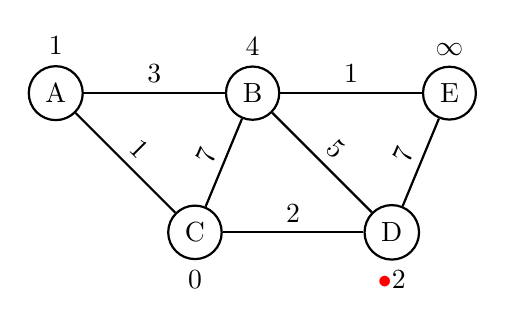
\begin{tikzpicture}[node distance={25mm}, thick, main/.style = {draw, circle}]
\node[main, label=above:{$\textcolor{green}{\checkmark}1$}] (1) {A};
\node[main, label=above:{$4$}] (2) [right of=1] {B};
\node[main, label=below:{$\textcolor{green}{\checkmark} 0$}] (3) [below right of=1] {C};
\node[main, label=below:{$\textcolor{red}{\bullet}2$}] (4) [below right of=2] {D};
\node[main, label=above:{$\infty$}] (5) [right of=2] {E};
\draw (1) -- node[midway, above, pos=0.5] {3} (2);
\draw (1) -- node[midway, above, sloped, pos=0.5] {1} (3);
\draw (2) -- node[midway, above, sloped, pos=0.5] {7} (3);
\draw (3) -- node[midway, above , pos=0.5] {2} (4);
\draw (2) -- node[midway, above, sloped, pos=0.5] {5} (4);
\draw (2) -- node[midway, above , pos=0.5] {1} (5);
\draw (4) -- node[midway, above, sloped, pos=0.5] {7} (5);
\end{tikzpicture}
\caption{Etape 4}\label{fig:etp_4}
\end{figure}
Nous répétons à nouveau l'algorithme. Cette fois, nous vérifions B et E.

Pour B, nous obtenons 2 + 5 = 7. Nous comparons cette valeur avec la distance minimale de B (4) et laissons la plus petite valeur (4). Pour E, nous obtenons 2 + 7 = 9, nous la comparons avec la distance minimale de E (infini) et nous laissons la plus petite (9).

Nous marquons D comme visité et mettons notre noeud actuel à B.
Regardez la figure~\ref{fig:etp_5}.
\begin{figure}[!htb]
\centering
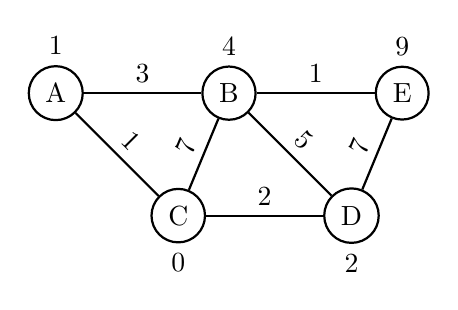
\begin{tikzpicture}[node distance={22mm}, thick, main/.style = {draw, circle}]
\node[main, label=above:{$\textcolor{green}{\checkmark}1$}] (1) {A};
\node[main, label=above:{$4$}] (2) [right of=1] {B};
\node[main, label=below:{$\textcolor{green}{\checkmark} 0$}] (3) [below right of=1] {C};
\node[main, label=below:{$\textcolor{green}{\checkmark}2$}] (4) [below right of=2] {D};
\node[main, label=above:{$9$}] (5) [right of=2] {E};
\draw (1) -- node[midway, above, pos=0.5] {3} (2);
\draw (1) -- node[midway, above, sloped, pos=0.5] {1} (3);
\draw (2) -- node[midway, above, sloped, pos=0.5] {7} (3);
\draw (3) -- node[midway, above , pos=0.5] {2} (4);
\draw (2) -- node[midway, above, sloped, pos=0.5] {5} (4);
\draw (2) -- node[midway, above , pos=0.5] {1} (5);
\draw (4) -- node[midway, above, sloped, pos=0.5] {7} (5);
\end{tikzpicture}
\caption{Etape 5}\label{fig:etp_5}
\end{figure}

Nous répétons l'algorithme pour chaque noeud et à la fin nous obtenons le graphe
de  la figure~\ref{fig:final_graph}.
\begin{figure}[!htb]
\centering
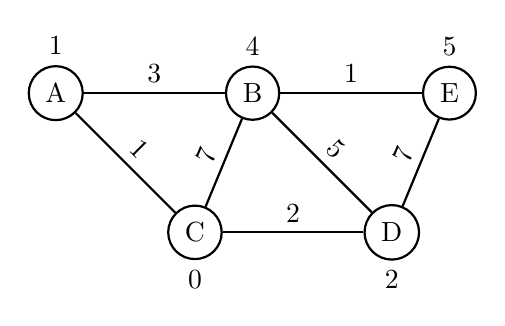
\begin{tikzpicture}[node distance={25mm}, thick, main/.style = {draw, circle}]
\node[main, label=above:{$\textcolor{green}{\checkmark}1$}] (1) {A};
\node[main, label=above:{$\textcolor{green}{\checkmark}4$}] (2) [right of=1] {B};
\node[main, label=below:{$\textcolor{green}{\checkmark}0$}] (3) [below right of=1] {C};
\node[main, label=below:{$\textcolor{green}{\checkmark}2$}] (4) [below right of=2] {D};
\node[main, label=above:{$\textcolor{green}{\checkmark}5$}] (5) [right of=2] {E};
\draw (1) -- node[midway, above, pos=0.5] {3} (2);
\draw (1) -- node[midway, above, sloped, pos=0.5] {1} (3);
\draw (2) -- node[midway, above, sloped, pos=0.5] {7} (3);
\draw (3) -- node[midway, above , pos=0.5] {2} (4);
\draw (2) -- node[midway, above, sloped, pos=0.5] {5} (4);
\draw (2) -- node[midway, above , pos=0.5] {1} (5);
\draw (4) -- node[midway, above, sloped, pos=0.5] {7} (5);
\end{tikzpicture}
\caption{Graphe finale}\label{fig:final_graph}
\end{figure}
Pour plus d'information~\cite{example.web}.
